\documentclass[11pt,a4paper]{report}
\usepackage[top=1in, bottom=1.5in, left=1in, right=1in]{geometry}
\usepackage[utf8]{inputenc}
\usepackage{amsmath}
\usepackage{amsfonts}
\usepackage{amssymb}
\usepackage[spanish,activeacute]{babel}
\usepackage{multirow}
\usepackage{graphicx}
\usepackage{setspace}
\usepackage{color}
\definecolor{red}{rgb}{1,0,0}
\newcommand\red[1]{\textcolor{red}{#1}}
\newcommand{\dsum}{\displaystyle\sum}

\begin{document}

\setlength{\unitlength}{1 cm} %Especificar unidad de trabajo
\thispagestyle{empty}
\begin{picture}(18,4)
\put(0,0){
\includegraphics[width=2.3cm,height=3cm]{LOGO.jpg}}
%\put(11.5,0){\includegraphics[width=4cm,height=4cm]{eupinf.jpg}}
\end{picture}
\begin{center}
\textbf{{\LARGE Universidad de Concepci\'on}}\\[0.5cm]
{\Large Facultad de Ciencias F\'isicas y Matem\'aticas}\\[0.5cm]
{\Large Departamento de Estad\'istica}\\[3.5cm]
{\LARGE \textbf{LABORATORIO III}}\\[1cm]
{\LARGE \textbf{DATA MINING}}\\ [4cm]
{\large Nombres: Katerin De la hoz Luna}\\
\hspace{2.2cm}{\large Fernando Pe\~na Villalobos}\\
\hspace{1.7cm}{\large Ariel P\'erez Almonacid}\\[2cm]

{\large Concepci\'on \\
\today}
\end{center}

\newpage

\begin{center}
Utilizando Rattle
\end{center}

\begin{itemize}
\item[1)]
\item[1.1)] El paso inicial es el mismo que en el laboratorio anterior, usando rattle() e importando la tabla SAheart, donde se buscará predecir qué pacientes poseen una enfermedad coronaria a partir de los otros datos que hay en la tabla:
\begin{center}
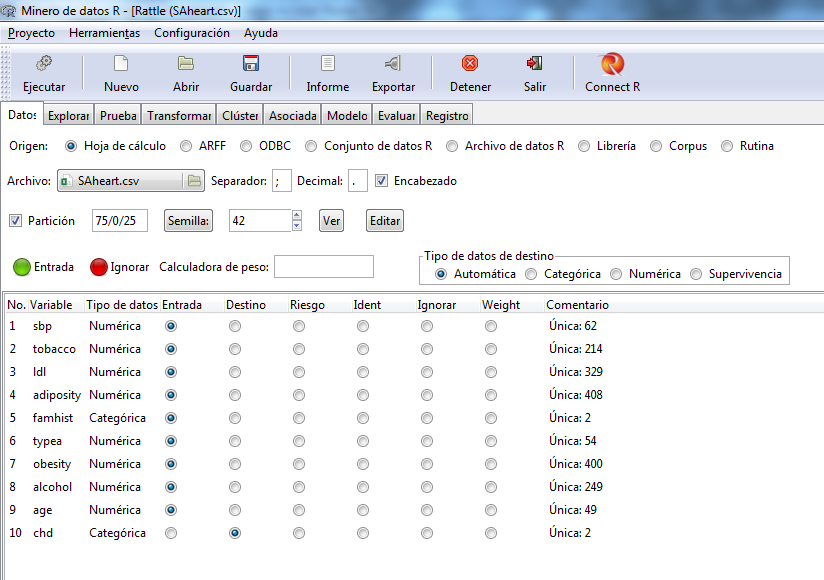
\includegraphics[scale=0.6]{4-1.png}
\end{center}
Ahora, yendo a Modelo, se marca SVM, ocupando en este caso Núcleo: Radial Basis, y se ejecuta.

\begin{verbatim}
Resumen del modelo SVM (construido con ksvm):

Support Vector Machine object of class "ksvm" 

SV type: C-svc  (classification) 
 parameter : cost C = 1 

Gaussian Radial Basis kernel function. 
 Hyperparameter : sigma =  0.105041657530422 

Number of Support Vectors : 236 

Objective Function Value : -181.8399 
Training error : 0.196532 
Probability model included. 

Tiempo transcurrido: 0.16 segs
\end{verbatim}

\item[1.2)] Para calcular la matriz de confusión, se cambia a la pestaña Evaluar, marcando en Matriz de Error y en SVM, el cual es el modelo con el que se está trabajando, y nuevamente se ejecuta, dando como resultado la siguiente matriz de confusión:
\begin{verbatim}
	      Predicho
Real   No 	Si
  No   67 	 9
  Si   23 	17
\end{verbatim}
De donde se puede extraer la siguiente información:\\
Precisión Global = $72\%$\\
Precisión Positiva = $43\%$\\
Precisión Negativa = $88\%$\\
Falsos Positivos = $12\%$\\
Falsos Negativos = $58\%$\\

Si se comparan estos resultados con los obtenidos utilizando árbol, cuya matriz de confusión es:
\begin{verbatim}
      Predicho
Real   No 	 Si
  No   55	 21
  Si   24 	 16
\end{verbatim}
Y los indicadores son los siguientes:\\
Precisión Global = $61\%$\\
Precisión Positiva = $40\%$\\
Precisión Negativa = $72\%$\\
Falsos Positivos = $28\%$\\
Falsos Negativos = $60\%$\\

se puede observar que en este caso es más conveniente utilizar Máquinas de Soporte Vectorial, con el kernel elegido, debido a que nos interesa tener un porcentaje bajo de falsos negativos. En este caso, se tiene un 58\% versus un 60\%, respectivamente.

\item[1.3)] Para graficar la curva ROC, en la misma pestaña, se marca ROC y el tipo de modelo con el que se desea graficar esta curva (en este caso, Árbol y SVM).
\begin{center}
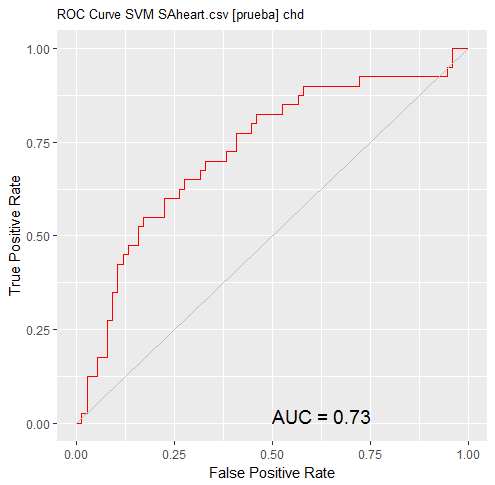
\includegraphics[scale=0.8]{SVM1.png}\\
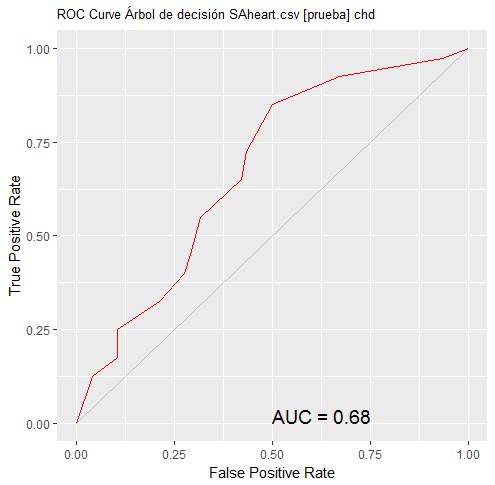
\includegraphics[scale=0.8]{arbold.png}
\end{center}
Aquí se observa que, juzgando por el área bajo la curva ROC, para ambos casos se obtiene un resultado decente, siendo más conveniente el método de Máquinas de Soporte Vectorial (AUC=0.73) que el de árboles de decisión (AUC=0.68). Sin embargo, como ya se comentó, lo principal a tomar en cuenta en este caso es cuál método minimiza el porcentaje de falsos negativos, por lo que, a pesar de que en este caso coincidan, es más conveniente quedarse con el criterio anterior para este problema.

\item[1.4)] Se regresa a la pestaña modelo y se ejecuta cambiando el Núcleo, según cuál se quiera ocupar. Para cada uno de los núcleos considerados, se obtuvieron las siguientes matrices de confusión:
\begin{verbatim}
Polynomial:
   	 Predicho
Real  No Si
  No  61 15
  Si  17 23
 			 
Linear:
			     Predicho
			Real  No Si
			  No  61 15
			  Si  17 23 	
			  
Hyperbolic Tangent:
 	  Predicho
Real  No Si
  No  61 15
  Si  20 20		
 			  
Laplacian:
    			 Predicho
			Real  No Si
			  No  68  8
			  Si  23 17 		
			  
Bessel:
			     Predicho
			Real  No Si
			  No  65 11
			  Si  23 17		
			  
ANOVA RBF:
			     Predicho
			Real  No Si
			  No  45 31
			  Si  19 21
			  
Spline:
			     Predicho
			Real  No Si
			  No  55 21
			  Si  20 20			  			  	  	  	  		 
\end{verbatim}
Para estos, se calcula el porcentaje de falsos negativos, que es el indicador de interés:\\
Polynomial = 43\%\\
Linear = 43\%\\
Hyperbolic Tangent = 50\%\\
Laplacian = 58\%\\
Bessel = 58\%\\
ANOVA RBF = 48\%\\
Spline = 50\%\\
Así, el método más conveniente para este caso es Máquinas de Soporte Vectorial, escogiendo Núcleo Polynomial o Núcleo Linear.\\



\begin{center}
Utilizando código
\end{center}

\item[1)]
\noindent Utilizando el código anexado, se procede en busca del mismo objetivo, y se empieza por ejecutar el modelo de Máquinas de Soporte Vectorial con Núcleo radial y se compara con lo realizado con Árboles de Decisión a través de la matriz de confusión:
\begin{verbatim}
Radial:
	      Predicho
Real   No 	Si
  No   71 	 9
  Si   23 	12
  
Árboles:
	      Predicho
Real   No 	Si
  No   63 	17
  Si   17 	18  
\end{verbatim}
Para SVM se tiene:\\
Precisión Global = $72\%$\\
Precisión Positiva = $34\%$\\
Precisión Negativa = $89\%$\\
Falsos Positivos = $11\%$\\
Falsos Negativos = $66\%$\\
\\
Para árboles de decisión se tiene:\\
Precisión Global = $70\%$\\
Precisión Positiva = $51\%$\\
Precisión Negativa = $79\%$\\
Falsos Positivos = $21\%$\\
Falsos Negativos = $49\%$\\
\\
En esta ocasión, dado que los datos de aprendizaje y prueba fueron elegidos distintos a los usados con el comando Rattle, nos conviene más usar árboles de decisión, ya que el porcentaje de falsos negativos es menor.\\
Por otro lado, las curvas ROC que resultan de estos modelos son las siguientes:
\begin{center}
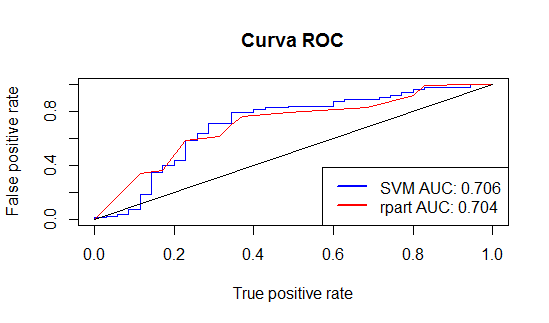
\includegraphics[scale=0.8]{4-1b.png}\\
\end{center}
Nuevamente, según estos gráficos, el mejor modelo vendría siendo la Máquina de Soporte Vectorial con núcleo radial. Sin embargo, como ya se mencionó, en este caso se conviene juzgar según lo hecho en el paso anterior.\\
\\
Ahora se procede a utilizar tres modelos más de Máquinas de Soporte Vectorial, pero utilizando otros núcleos. 
\begin{verbatim}  
Polynomial:
	      Predicho
Real   No 	Si
  No   75 	 5
  Si   19 	16
  
Lineal:
	      Predicho
Real   No 	Si
  No   70 	10
  Si   19 	16

Hyperbolic Tangent:
	      Predicho
Real   No 	Si
  No   65 	15 
  Si   21 	14
\end{verbatim}
cuyos porcentajes de falsos negativos son:\\
Polynomial = 54\%\\
Linear = 54\%\\
Hyperbolic Tangent = 60\%\\

De aquí se vuelve a apreciar un mejor resultado para el caso de los núcleos Linear y Polynomial (siendo el árbol en esta ocasión mejor que ambos).\\

\end{itemize}
\begin{center}
Utilizando Rattle
\end{center}


\begin{itemize}
\item[3)]
\item[3.1)] Luego de probar el método de Máquinas de Soporte Vectorial con varios núcleos, el criterio para escoger el mejor fue comparar tiempo de ejecución y precisión global:\\

\begin{tabular}{|l|c|c|}
\hline 
Núcleo & Tiempo de ejecución (segs) & precisión global (\%)\\
\hline
Radial basis & 43.67 & 94 \\
\hline 
Plynomial & 22.02 & 93 \\
\hline 
Linear & 15.50 & 93 \\
\hline 
Hyperbolic Tangent & 116.40 & 36 \\
\hline 
Laplacian & 117.60 & 90 \\
\hline
Bessel & 535.80 & 7 \\
\hline
\end{tabular} \\

Así, se escoge el núcleo linear, ya que tiene el menor tiempo de ejecución y una de las más altas precisiones globales. \\
En el caso de árbol de decisión, el tiempo fue de 17.9 segs y la precisión de 73\%. 
\item[3.2] La matriz de confusión para SVM con núcleo linear es la siguiente:
\begin{verbatim}
         Predicho
 Real    cero cinco cuatro dos nueve ocho seis siete tres uno
  cero    351     0      2   3     0    1    2     0    0   0
  cinco     5   141      2   0     2    3    0     0    7   0
  cuatro    2     2    181   5     4    0    2     2    0   2
  dos       3     5      3 179     0    3    1     1    3   0
  nueve     0     1      2   0   171    0    0     3    0   0
  ocho      7     4      0   4     3  144    0     0    4   0
  seis      0     2      4   2     0    1  161     0    0   0
  siete     0     0      6   1     5    1    0   134    0   0
  tres      2     9      0   2     0    4    0     1  148   0
  uno       0     0      5   0     1    1    3     0    0 254
\end{verbatim}
Y las precisiones positivas para cada número son: \\
cero = 98\%\\
cinco = 89\%\\
cuatro = 91\%\\
dos = 90\%\\
nueve = 97\%\\
ocho = 87\%\\
seis = 95\%\\
siete = 91\%\\
tres = 89\%\\
uno = 96\%\\
\\
Así, estos indicadores y lo obtenido en la parte 1, permiten concluir que es mejor utilizar SVM, con el núcleo escogido, que árbol de decisión. \\ \\
Los números con las precisiones positivas más bajas, para el caso de SVM, son el ocho, cuatro y dos, que aún así poseen valores altos. En el caso de árbol de decisión, estos números también tuvieron bajos porcentajes del indicador. El ocho se confundió mucho con el cero, el cuatro con el dos y el nueve, y el dos con el cinco. La principal razón de que estos números inducen una menor precisión tiene que ver con su forma; las curvas que los caracterizan y las distintas maneras de escribirlos.
\item[3.3)] Como existen más de dos clases, es decir, el problema no es del tipo clasificación binaria, no es posible obtener la curva ROC; y por lo tanto, la única forma de analizar el modelo de SVM, y compararlo con árbol de decisión, es midiante los indicadores descritos anteriormente.

\begin{center}
 Utilizando código
\end{center}
\item[3)]
Como las tablas de aprendizaje y de prueba están previamente establecidas, los resultados usando rattle y usando código no varían significativamente (a diferencia del problema 1, donde la manera en la que los datos totales son divididos si genera cambios en los resultados). \\
La matrices de confusión, y los indicadores de interés, con el modelo SVM, son los siguientes:
\begin{verbatim}
        prediccionsvm
         cero cinco cuatro dos nueve ocho seis siete tres uno
  cero    348     0      3   3     0    1    4     0    0   0
  cinco     5   141      2   0     1    3    0     1    7   0
  cuatro    1     2    180   5     4    0    4     2    0   2
  dos       1     4      3 178     0    3    2     1    6   0
  nueve     0     1      2   0   171    0    0     3    0   0
  ocho      5     4      0   1     1  147    1     0    7   0
  seis      0     2      4   1     0    1  162     0    0   0
  siete     0     0      6   1     4    1    0   135    0   0
  tres      2     9      0   2     0    4    0     1  148   0
  uno       0     0      5   0     0    0    3     0    0 256
\end{verbatim}
Precisión global = 93\% 

Precisiones positivas para cada número: \\
cero = 97\%\\
cinco = 88\%\\
cuatro = 90\%\\
dos = 90\%\\
nueve = 97\%\\
ocho = 89\%\\
seis = 95\%\\
siete = 92\%\\
tres = 89\%\\
uno = 97\%\\

Para el caso de árbol de decisión, tampoco se obtienen resultados significativamente distintos a los obtenidos con rattle, por la misma razón dada anteriormente. La matriz de confusión y los indicadores de interés son los siguientes:

\begin{verbatim}
        prediccionrpart
         cero cinco cuatro dos nueve ocho seis siete tres uno
  cero    294     2      1  31     0   15    1     0   12   3
  cinco    17    89      2   6     1    7   10     2   15  11
  cuatro    1     1    138  11    13    5    0     5    0  26
  dos       9     2     13 111     4   24   11     5   10   9
  nueve     0     0      1   2   138    7    0     8    5  16
  ocho      1     3      2  11     5  120    1     2   12   9
  seis     11    10      2   4     0   27  104     3    1   8
  siete     0     1     10   6     4    3    0   113    1   9
  tres     10    22      3   2     1   16    0     3  105   4
  uno       1     1      3   2     8    5    0     1    0 243
\end{verbatim}
Precisión global = 72\%

Precisiones positivas para cada número:\\
cero = 82\%\\
cinco = 56\%\\
cuatro = 69\%\\
dos = 56\%\\
nueve = 78\%\\
ocho = 72\%\\
seis = 61\%\\
siete = 77\%\\
tres = 63\%\\
uno = 92\%\\
\end{itemize}

\begin{center}
ANEXO:
\end{center}

\begin{itemize}
\item[1)]
Máquinas de Soporte Vectorial con Núcleo Radial y Árboles de Decisión:

\begin{verbatim} 
Datos<-read.table('SAheart.csv', sep=";", dec=".", header=T) 
head(Datos)

##Fijamos la semilla de modo de poder comparar los resultados
set.seed(30)

#Generamos una muestra donde el 75% de los datos serán utilizados como 
#tabla de aprendizaje y el 25% como tabla de prueba (testing):
muestra <-sample(1:nrow(Datos),nrow(Datos)%/%(100/25)) 
ttesting<-Datos[muestra,]
taprendizaje<- Datos[-muestra,]

#Generamos el modelo utilizando la función kernel radial:
modelosvm<-svm(chd~.,data=taprendizaje, kernel="radial") 

#Realizamos las predicciones sobre la tabla de prueba:
prediccionsvm<-predict(modelosvm, ttesting) 

#Calculamos la matriz de confusión y la precisión global:
MCsvm<-table(ttesting[,ncol(Datos)],prediccionsvm) 
MCsvm
PGsvm<-(sum(diag(MCsvm)))/sum(MCsvm)
PGsvm

#Comparativa con árboles de decisión

modelorpart<-rpart(chd~.,data=taprendizaje)
prediccionrpart<-predict(modelorpart, ttesting, type="class")
MCrpart<-table(ttesting[,ncol(Datos)],prediccionrpart) 
MCrpart
PGrpart<-(sum(diag(MCrpart)))/sum(MCrpart)
PGrpart

#El siguiente código permite construir la curva ROC 
#sin la necesidad de recurrir a rattle:
modelosvm<-svm(chd~.,data=taprendizaje, kernel="radial", probability=TRUE)
modelorpart<-rpart(chd~.,data=taprendizaje)

prediccionsvm<-predict(modelosvm, ttesting, probability=TRUE)
prediccionrpart<-predict(modelorpart, ttesting, probability=TRUE)

prediccionsvm.rocr <- prediction(attr(prediccionsvm, "probabilities")[,2], ttesting$chd)
prediccionrpart.rocr <- prediction(prediccionrpart[,1], ttesting$chd)

prediccionsvm.perf <- performance(prediccionsvm.rocr, "fpr", "tpr")
prediccionrpart.perf <- performance(prediccionrpart.rocr, "fpr", "tpr" )

plot(prediccionsvm.perf, main="Curva ROC", col="blue")
plot(prediccionrpart.perf, col="red", add=TRUE)
lines(c(0,1), c(0,1), col="black")

#El área bajo la curva, AUC, está dada por:
AUCsvm<-1-as.numeric(slot(performance(prediccionsvm.rocr,"auc"), "y.values"))
AUCsvm

AUCrpart<-1- as.numeric(slot(performance(prediccionrpart.rocr,"auc"), "y.values"))
AUCrpart

legend("bottomright", c(paste("SVM", "AUC:",round(AUCsvm, 3)), 
                        paste("rpart", "AUC:", round(AUCrpart,3))), 
       lty = c(1,1), lwd=c(2.5,2.5),col=c("blue","red"))
\end{verbatim}

Máquinas de Soporte Vectorial usando núcleo:

\item Polinomial:
 

\begin{verbatim} 

set.seed(30)

#Generamos una muestra donde el 75% de los datos serán utilizados como 
#tabla de aprendizaje y el 25% como tabla de prueba (testing):
muestra <-sample(1:nrow(Datos),nrow(Datos)%/%(100/25)) 
ttesting<-Datos[muestra,]
taprendizaje<- Datos[-muestra,]

#Generamos el modelo utilizando la función kernel polinomial:
modelosvm<-svm(chd~.,data=taprendizaje, kernel="polynomial") 

#Realizamos las predicciones sobre la tabla de prueba:
prediccionsvm<-predict(modelosvm, ttesting) 

#Calculamos la matriz de confusión y la precisión global:
MCsvm<-table(ttesting[,ncol(Datos)],prediccionsvm) 
MCsvm
PGsvm<-(sum(diag(MCsvm)))/sum(MCsvm)
PGsvm

#Generamos el modelo utilizando la función kernel polinomial:
modelosvm<-svm(chd~.,data=taprendizaje, kernel="polynomial") 

#Realizamos las predicciones sobre la tabla de prueba:
prediccionsvm<-predict(modelosvm, ttesting) 

#Calculamos la matriz de confusión y la precisión global:
MCsvm<-table(ttesting[,ncol(Datos)],prediccionsvm) 
MCsvm
PGsvm<-(sum(diag(MCsvm)))/sum(MCsvm)
PGsvm

\end{verbatim}

\item Lineal:
\begin{verbatim} 

set.seed(30)

#Generamos una muestra donde el 75% de los datos serán utilizados como 
#tabla de aprendizaje y el 25% como tabla de prueba (testing):
muestra <-sample(1:nrow(Datos),nrow(Datos)%/%(100/25)) 
ttesting<-Datos[muestra,]
taprendizaje<- Datos[-muestra,]

#Generamos el modelo utilizando la función kernel lineal:
modelosvm<-svm(chd~.,data=taprendizaje, kernel="linear") 

#Realizamos las predicciones sobre la tabla de prueba:
prediccionsvm<-predict(modelosvm, ttesting) 

#Calculamos la matriz de confusión y la precisión global:
MCsvm<-table(ttesting[,ncol(Datos)],prediccionsvm) 
MCsvm
PGsvm<-(sum(diag(MCsvm)))/sum(MCsvm)
PGsvm

#Generamos el modelo utilizando la función kernel lineal:
modelosvm<-svm(chd~.,data=taprendizaje, kernel="linear") 

#Realizamos las predicciones sobre la tabla de prueba:
prediccionsvm<-predict(modelosvm, ttesting) 

#Calculamos la matriz de confusión y la precisión global:
MCsvm<-table(ttesting[,ncol(Datos)],prediccionsvm) 
MCsvm
PGsvm<-(sum(diag(MCsvm)))/sum(MCsvm)
PGsvm

\end{verbatim}
\item Hyperbolic tangent:
\begin{verbatim} 

set.seed(30)

#Generamos una muestra donde el 75% de los datos serán utilizados como 
#tabla de aprendizaje y el 25% como tabla de prueba (testing):
muestra <-sample(1:nrow(Datos),nrow(Datos)%/%(100/25)) 
ttesting<-Datos[muestra,]
taprendizaje<- Datos[-muestra,]

#Generamos el modelo utilizando la función kernel Hyperbolic Tangent:
modelosvm<-svm(chd~.,data=taprendizaje, kernel="sigmoid") 

#Realizamos las predicciones sobre la tabla de prueba:
prediccionsvm<-predict(modelosvm, ttesting) 

#Calculamos la matriz de confusión y la precisión global:
MCsvm<-table(ttesting[,ncol(Datos)],prediccionsvm) 
MCsvm
PGsvm<-(sum(diag(MCsvm)))/sum(MCsvm)
PGsvm

#Generamos el modelo utilizando la función kernel Hyperbolic Tangent:
modelosvm<-svm(chd~.,data=taprendizaje, kernel="sigmoid") 

#Realizamos las predicciones sobre la tabla de prueba:
prediccionsvm<-predict(modelosvm, ttesting) 

#Calculamos la matriz de confusión y la precisión global:
MCsvm<-table(ttesting[,ncol(Datos)],prediccionsvm) 
MCsvm
PGsvm<-(sum(diag(MCsvm)))/sum(MCsvm)
PGsvm

\end{verbatim}

\item[3)] Máquina de Soporte Vectorial con Núcleo Linear y Árboles de decisión:
\begin{verbatim}
#Cargamos la tabla de entrenamiento y de testeo
train <- read.csv("ZipDataTrainCod.csv", sep = ";", dec = ".", header = T)
head(train)
test <- read.csv("ZipDataTestCod.csv", sep = ";", dec = ".", header = T)
head(test)

#Generamos el modelo SVM con núcleo linear
modelosvm <- svm(Numero~., data = train, kernel = "linear")

#Realizamos las predicciones sobre la tabla de testeo
prediccionsvm <- predict(modelosvm, test)

#Calculamos la matriz de confusion y la precision global
MCsvm <- table(test[,1], prediccionsvm)
MCsvm
PGsvm <- (sum(diag(MCsvm)))/(sum(MCsvm))
PGsvm

#Precisiones positivas

x <- rep(0,10)
y <- c("cero","cinco","cuatro","dos","nueve","ocho","seis","siete","tres","uno")
PrecPossvm <- data.frame(y,x)
PrecPossvm <- as.matrix(PrecPossvm)

for (i in 1:10){
  PrecPossvm[i,2] <- round(((MCsvm[i,i])/(sum(MCsvm[i,])))*100)
  
}
PrecPossvm

#Comparativa con árbol de decisión
modelorpart <- rpart(Numero~., data = train)
prediccionrpart <- predict(modelorpart, test, type = "class")
MCrpart <- table(test[,1], prediccionrpart)
MCrpart
PGrpart <- (sum(diag(MCrpart)))/(sum(MCrpart))
PGrpart

PrecPosrpart <- data.frame(y,x)
PrecPosrpart <- as.matrix(PrecPosrpart)

for (i in 1:10){
  PrecPosrpart[i,2] <- round(((MCrpart[i,i])/(sum(MCrpart[i,])))*100)
  
}
PrecPosrpart

\end{verbatim}


\end{itemize}

\end{document}
